\documentclass[a4paper,doc]{apa6}

\usepackage{hyperref}
\usepackage[american]{babel}

% references:
\usepackage{csquotes}
\usepackage[style=apa6,backend=biber]{biblatex}
\DeclareLanguageMapping{american}{american-apa}
\addbibresource{arangodb.bib}

% abbreviations:
\usepackage[acronym]{glossaries}

% code snippets:
\usepackage{listings}
\usepackage[dvipsnames]{xcolor}
\definecolor{ListingBackground}{HTML}{F8F8F8}
\lstset{
  basicstyle=\ttfamily\footnotesize,
  keywordstyle=\color{blue}\ttfamily,
  stringstyle=\color{red}\ttfamily,
  commentstyle=\color{green}\ttfamily,
  morecomment=[l][\color{magenta}]{\#},
  frame=single,			        % border settings
  frameround=ffff,
  rulecolor=\color{darkgray}, % border color,
  captionpos=b,			% sets the caption-position to bottom
  xleftmargin=10pt,		        % margin left
  xrightmargin=5pt,		        % margin right
  showstringspaces=false,
}

\definecolor{ArangoKeywordColor}{HTML}{0600ff}
\definecolor{ArangoFuncColor}{HTML}{3c4b72}
\definecolor{ArangoStringColor}{HTML}{036a06}
\definecolor{ArangoNumberColor}{HTML}{0300cd}
\lstdefinelanguage{ArangoQL}{
  sensitive=false,
  morekeywords={FOR,IN,FILTER,OUTBOUND,RETURN,SORT,
    LIMIT,SEARCH,ASC,DESC,COLLECT,INTO,LET,AND,
    UPDATE,WITH
  },
  keywordstyle=\color{ArangoKeywordColor},
  morekeywords={[2]PHRASE,ANALYZER,STARTS_WITH,
    TFIDF,BM25,TOKENS,MINUS,DOCUMENT,UNION,MERGE,
    DATE_ISO8601,LENGTH,FLATTEN,UNIQUE,CONCAT
  },
  keywordstyle=[2]\color{ArangoFuncColor},
  morestring=[b]",
  morestring=[b]',
  stringstyle=\color{ArangoStringColor},
  numberstyle=\color{ArangoNumberColor},
}


\makenoidxglossaries{}
\newacronym{aql}{AQL}{ArangoDB Query Language}
\newacronym{tf-idf}{TF-IDF}{Term Frequence-Inverse Document Frequency}


\title{ArangoDB}
\shorttitle{ArangoDB}
\date{\today}

\author{7695507, 3711191 and 8786673}
\affiliation{New DB Technologies -- Duale Hochschule Baden-Württemberg, Stuttgart}

\keywords{ArangoDB, database, multi-model, NoSQL, graph}

\abstract{ArangoDB is NoSQL database with a multi-model paradigm. In this paper we will demonstrate its characteristics and features. We will compare it with traditional SQL mechanisms and with other NoSQL databases.}

\begin{document}
\maketitle

\tableofcontents

%!TEX root = ./main.tex

\section{Introduction: Multi-Model Databases}

\section{ArangoDB in distributed systems}

\section{Installation}

Upon Installation you have the choice between two Storage Engines – MMFiles and RocksDB. `The MMFiles Storage Engine is deprecated starting with version 3.6.0 and will be removed in a future release' \cite{ArangoDeprecated}.

This is due to a few downsides on part of the MMFiles engine. It only supports data set that fit in its entirety into memory. It also does not support concurrency in reading writing locking on a collection (table) level. RocksDB enables concurrent reads and writes. This can lead to exceptions that need to be handled. RocksDB persists indexes on disk and therefore has a faster startup time. What's important to note is that it puts an upper limit on the transaction size, because it is optimized for smaller transactions. Transactions that are too large will be split into multiple smaller commits automatically which might violate ACID properties. This limit can be re-configured. In future Arango plans to handle large transactions as a series of small transactions which will remove the size restriction. \cite{MMvsRocks}

The ArangoDB installation comes with a pre-installed Web Dashboard that provides an overview over data collections, graphical output formatting for graph data as well as an editor for querying and manipulating data in the \gls{aql}. It also comes with a CLI that can be used for more advanced features and configurations such as data sharding. There are interfaces available to multiple high-level programming languages such as Python, Java or C++. 
%We tested the Python interface which comes in form of a PyPi package `python-arango`. We were able to create a new entry, but failed in updating exisiting documents, even after extensive research into possible problems.

\section{Demo}

\section{Multi-Model Functions}

ArangoDB's strength lies within its capabilities to combine very different paradigms and data models in \gls{aql}. We will present features for storing and querying graph data, optimized operation on geographical data and optimized information retrieval on natural language texts.

\subsection{Graph Data}

Besides to the normal document collections one can create Edge collections. Each entry in such a collection represents a directed edge and must have at least two properties: \texttt{from\_} and \texttt{to\_} which hold the keys of documents representing the nodes connected by the edge. The entries can also hold other attributes (e.g.\ weight or distance). 


\begin{figure}[thp]
\centering
\begin{lstlisting}[]
FOR c IN Characters
	FILTER c.name == "Bran"
	FOR parent in 1..2 OUTBOUND c ChildOf
		RETURN parent.name
\end{lstlisting}
\caption{Combining graph and relational data: Looks for a character and uses out-going edges of type \texttt{ChildOf} (= incoming edges of type \texttt{ParentOf}) to determine the character's parents and grandparents.}
\end{figure}


There exist functions for graph traversal or finding the k shortest paths from A to B. Latter requires the definition of which attribute in the edge entry to regard as the weight \cite{ShortestPath}.

\subsection{Geo Indexing}

Next to a primary index (key) a document collection can also hold a second index: a \texttt{GeoIndex}, which is defined on a document attribute that holds an array of length two representing the latitude and longitude of the location. A tutorial \cite{GeoTut} still demonstrates the Geo Index Functions \texttt{NEAR} that could be used to determine the N nearest locations to a certain point, and \texttt{WITHIN} that could be used to determine locations within a certain radius.
These are deprecated startimg from version 3.4.0 and were replaced by Geo utility functions, mainly the \texttt{DISTANCE} which can be used in combination with general \gls{aql} to achieve the same results as aforementioned functions. This queries will nonetheless still be optimized, as long as the attributes operated on have been marked as Geo Indexes \cite{GeoFunc}.

ArangoDB has extended the idea of two coordinates acting as a geo index to a more general geospatial format: \texttt{GeoJSON}. Next to geographic points it also among others allows the definition of \texttt{MultiLineString}s which could represent paths or routes and \texttt{Polygon}s which could represent areas or buildings \cite{GeoJSON}.
The functions \texttt{GEO\_CONTAINS}, \texttt{GEO\_AREA} or \texttt{GEO\_INTERSECTS} can then be used for evaluation of polygons in regards to whether it contains a certain point, the size of the area it circumfences or whether it intersects with a second polygon \cite{GeoFunc}.

\subsection{Information Retrieval}

Search in natural language texts can be a relevant, but complex and compute-expensive operation. Arango provides functions and optimizations that facilitate this task in the form of two methods: Fulltext indexing and ArangoSearch.

Equal to geo indexes an attribute within a document can be marked as a fulltext index. The attribute needs to contain a string, an object with string properties or an array of strings \cite{FulltextIndex}. This opens up the \texttt{FULLTEXT} functionality which allows to look for documents which do (not) contain or do (not) start with a certain word. These checks can be combined in conjunctions or disjunctions \cite{FulltextFunc}.

ArangoSearch is a search engine that was created to help in querying semi- or unstructured data and offers ranking mechanisms. It parses documents and creates an inverted index which holds a mapping for each word in vocubalry to each document in the corpus it is contained in. This enables quick queries and a naive ranking methodology: given a set of words in query return the document which holds most of these words.
This quite simple mechanism can be improved using known NLP methods: tokenization and stemming. ArangoDB overs text analyzers for many language that can split sentences into words (respecting cases like `aren\'t') and matching them to their according stem (e.g.\ jumps = jump). This enables the unified analysis of texts originating from multiple languages.
A further improvement can be the usage of more sophisticated ranking mechanisms than the described naive ranking. \gls{tf-idf} can be used to weight words according to their global importance (`is' is less important than `archaeopteryx').
The `BM25' metric combines the word's frequency within the text with its overall importance (\gls{tf-idf}), the length of the document and the average document length to determine a qualified measure that can be used to score a document's relevance to a given search query. \cite{ArangoSearchTut}

\begin{figure}[thp]
\centering
\begin{lstlisting}
FOR d IN v_imdb 
    SEARCH 
    ANALYZER(d.description IN 
                    TOKENS('amazing action world alien sci-fi science documental galaxy', 
                                 'text_en'),
                     'text_en')
    SORT BM25(d) DESC 
  LIMIT 10 
    RETURN d
\end{lstlisting}
\caption{Searching a database of movie descriptions}
\end{figure}



\appendix

\section{Figures}
\begin{figure}[h]
  \centering
  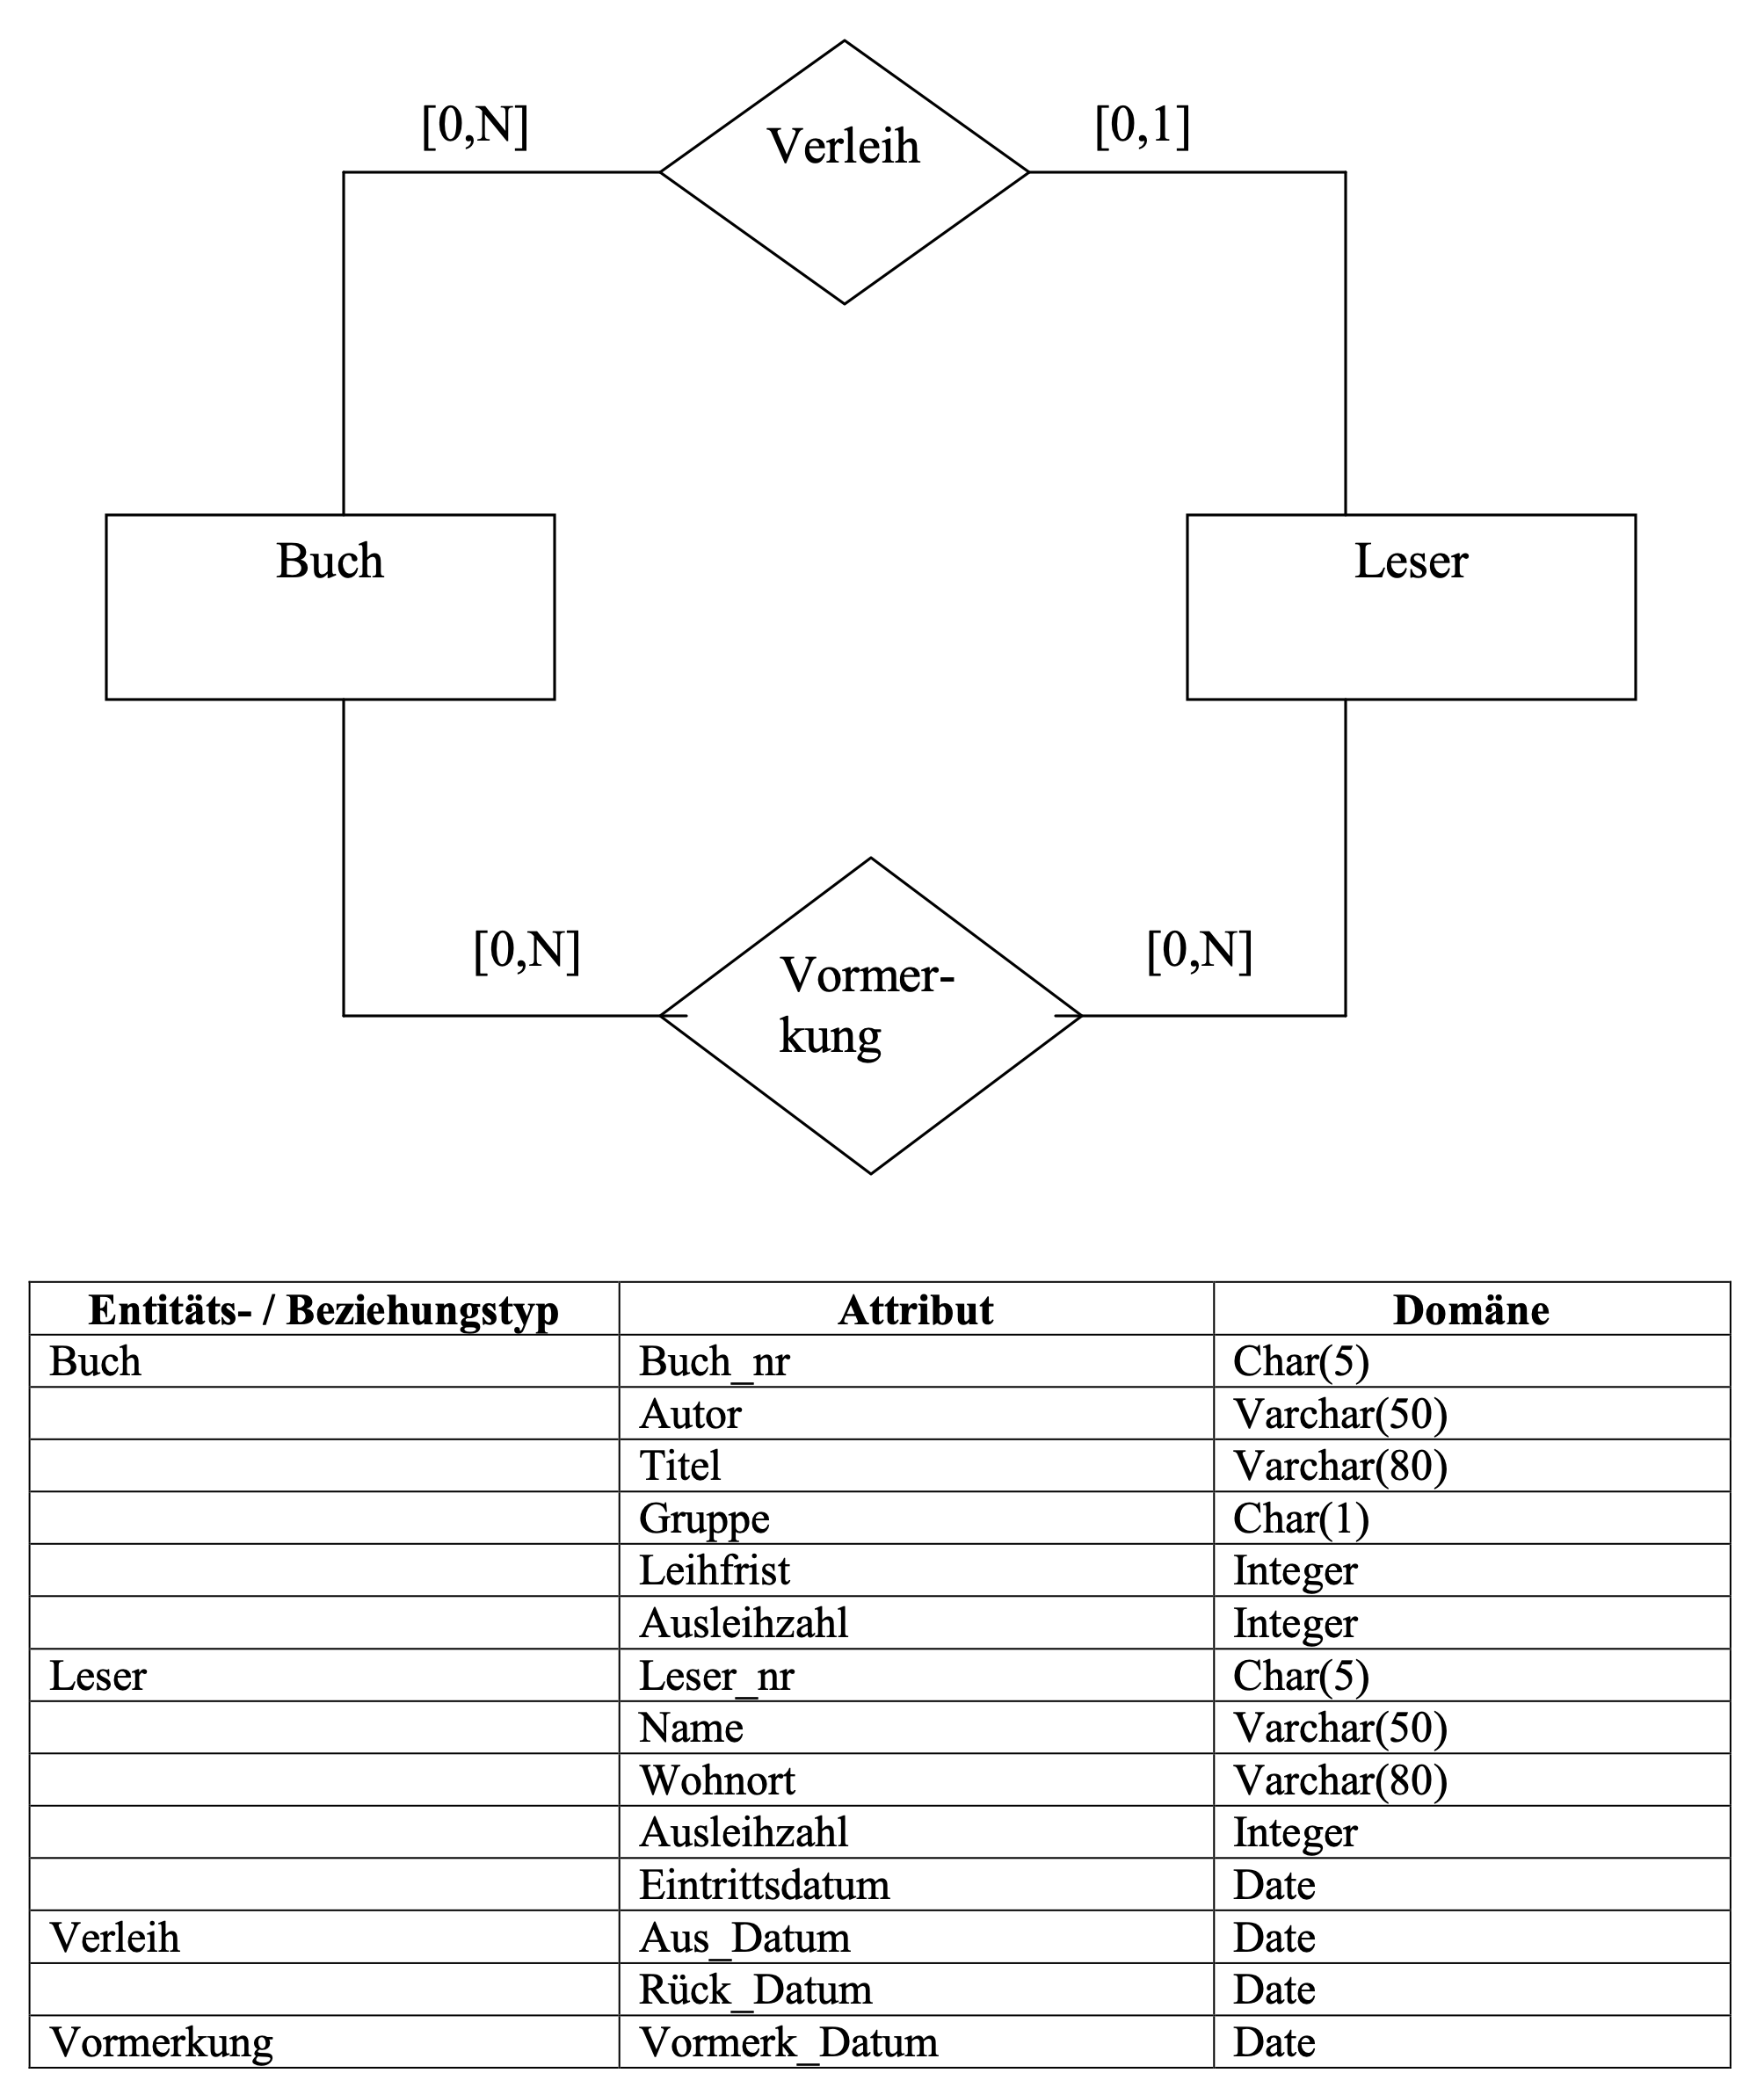
\includegraphics[width=0.9\textwidth]{images/erm.png}
  \caption{An examplary ERM of a book shop}
  \label{fig:book_shop_erm}
\end{figure}

\newpage
\printnoidxglossary[type=\acronymtype,numberedsection=autolabel]

\newpage
\printbibliography{}

\end{document}
